ue1:

1.Aufgabe:
\begin{equation}
\begin{split}
b \in \left\{ x_1 \cdot \begin{pmatrix*} 1\\ 1\\ 1 \end{pmatrix*} + x_2 \cdot \begin{pmatrix*} 1\\ -2\\ -1 \end{pmatrix*} | x_1, x_2 \in \R \right\}
\end{split}
\end{equation}
eine möglichst \glqq gute\grqq{} Lösung könnte sinnvollerweise foglendes erfüllen:

\[
\norm{Ax-b}^2_2 \longrightarrow min
\]

2.Aufgabe:
\begin{figure}[ht]
	\centering
	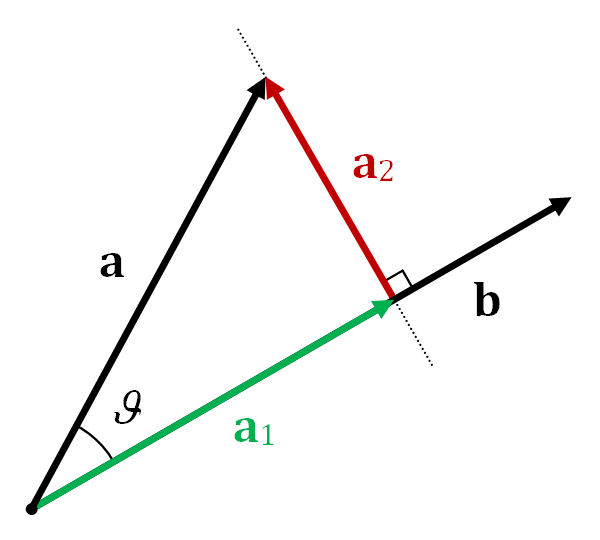
\includegraphics[scale=.3]{Projection_and_rejection.png}
\end{figure}

\begin{equation}\begin{split}
u = \begin{pmatrix*}1\\1\\1\end{pmatrix*}\quad;\quad
v = \begin{pmatrix*}0\\2\\1\end{pmatrix*}\\
v = v_{\bot} + v_{\parallel}\\\\
\end{split}\end{equation}
\begin{equation}\begin{split}
<v; u>
&= <v_{\bot} + v_{\parallel}; u>\\
&= <v_{\bot}; u> + <v_{\parallel}; u>\\
&= \cancelto{0}{<v_{\bot}; u>} \quad + <v_{\parallel}; u>\\
&= <v_{\parallel}; u>\\
\end{split}\end{equation}


5. Aufgabe:
\begin{equation}\begin{split}
f(t) &= \alpha \cos\left(\frac{\pi}{4}t\right) + \beta \sin\left(\frac{\pi}{3}t\right) \\
\varphi(t, \alpha, \beta) &= \alpha \cos\left(\frac{\pi}{4}t\right) + \beta \sin\left(\frac{\pi}{3}t\right)\\\\
\rightarrow & 
A = 
\begin{pmatrix*}
\cos\left(\frac{\pi}{4}1\right) & \sin\left(\frac{\pi}{3}1\right)\\
\cos\left(\frac{\pi}{4}2\right) & \sin\left(\frac{\pi}{3}2\right)\\
\cos\left(\frac{\pi}{4}3\right) & \sin\left(\frac{\pi}{3}3\right)\\		
\end{pmatrix*}\\
A &= 
\begin{pmatrix*}
\frac{1}{\sqrt{2}}  & \frac{\sqrt{3}}{2}\\
0                   & \frac{\sqrt{3}}{2}\\
-\frac{1}{\sqrt{2}} & 0\\		
\end{pmatrix*}
\quad, \quad
b = 
\begin{pmatrix*}
2\\
0\\
-3
\end{pmatrix*}
\end{split}\end{equation}

Normalengleichung:
\[
	A^T A x = A^T b
\]


